
\section{Aufbau}

Das Kugelfall-Viskosimeter besteht im großen und ganzen aus einem Rohr,
das die zu untersuchende Flüssigkeit enthält, umgeben von einem Gefäß,
in dem sich Wasser befindet, um die Flüssigkeit auf eine gewisse
Temperatur zu bringen, und einem Stativ, das die Apparatur drehbar
lagert. Die Temperatur des Wasserbads kann über ein Thermostat
eingestellt werden, das sich am Fuß des Gefäßes befindet.

Zusätzlich befindet sich noch ein Thermometer zur Messung der
Wasserbadtemperatur im Gefäß und eine Libelle am Stativ, mit der
sichergestellt werden kann, das die Apparatur gerade steht.

Auf dem Rohr, in das die Kugel zur Messung eingelegt wird, befinden sich
drei Marken. Eine Skizze ist in Abbildung~\ref{fig:aufbau} zu sehen.

\begin{figure}
  \centering
  \includegraphics{aufbau}
  \caption{Schema der verwendeten Apparatur}
  \label{fig:aufbau}
\end{figure}
